\documentclass{l4proj}

\usepackage{graphicx}
\usepackage{listings}
\usepackage{pdflscape}
\usepackage{pdfpages}
\usepackage{caption}
\usepackage{url}
\usepackage{cite}
\DeclareGraphicsExtensions{.pdf,.png,.jpg}

\pagenumbering{arabic}


\begin{document}
\title{Darwin: A Genetic Programming Framework for Cloning Web Services}
\author{George Kouzmov}
\date{31 January 2014}
\maketitle

\tableofcontents
\listoffigures
\listoftables
%==============================================================================
\chapter{Introduction}
In recent years web services have become a main method of communicating between applications
and accessing needed information, creating similar to a distributive environment for many developers.
Because of the standardized communication used by the web services they are expected to be used even 
more in the future providing even more commodities for both developers and users. The nature of web
services is a black box system which means we are unfamiliar with its contents and we only know how to
access it and what it returns. 
\paragraph{}
That's where the idea came from, for copying a web services using genetic
programming, which became a proof of concept project that reached very far. The genetic programming 
involves generating programs based on set of functions and then evaluating the quality (correctness)
of the program via a fitness function. To prove that cloning of a web service can be achieved using
genetic programming we used a symbolic regression problem where the genetic program needs to find a 
mathematical expression that yields the same result as a given one from a fitness function. But 
instead of using our own fitness function we are using a real web service hence generating a program
that has the same functionality as the web service. Proving this meant that theoretically by increasing 
the complexity of our function set we can achieve copying of an even more complex web service.


\section{What is Genetic Programming?}
Genetic programming is a branch of artificial intelligence inspired by biological evolution. It is a machine learning
technique that optimizes a population of computer programs until they start performing the user specified
functionality. Like the more widespread genetic algorithms (GA), genetic programming uses an evolutionary algorithm
based methodology to iterate through solutions until a correct one is found. In genetic programming a 
predefined size \textbf{population} is iterated through a user defined number of \textbf{generations}. 
The population consists of \textbf{individuals} which are programs represented as a tree structure.
This tree structure is constructed from a pre-defined set of \textbf{primitives} and \textbf{terminals}.
The primitives represent the functions from which the individual is constructed and
the terminals represent the bottom nodes of the tree, they can be both arguments and constants. A tree representation of an individual
can be seen in figure \ref{fig:ind}
\begin{figure}[htp]
\centering
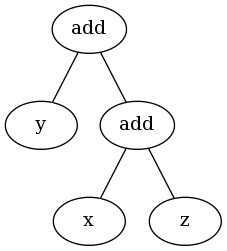
\includegraphics[scale=0.6]{Figures/ind.png}
\caption{An example of a genetic programming individual that represents x+y+z}
\label{fig:ind}
\end{figure}
A genetic program needs a \textbf{fitness function} through which each individual
is evaluated and compared. This way the correctness of the program can be calculated. Usually there are two type of fitness function 
minimum and maximum where minimum is looking for individuals with fitness values closer to 0 (where 0 usually means that a solution is found)
and maximum for the individuals with highest fitness result.
\paragraph{}
Genetic program randomly generates individuals for the first generation, evaluates them through the 
fitness function and creates new programs through \textbf{crossover} and \textbf{mutation}. Crossover 
is used to combine the genetic information of two individuals which means switching the nodes of a tree of one individual
with another as seen in figure \ref{fig:cross}. With a tree-based representation replacing a node means replacing the whole branch. When mutation
is applied to an individual a single node is replaced with a new randomly generated one. Changing a single
node can mean changing the whole branch shown in figure \ref{fig:mut}. After crossover and mutation are applied to the population a new generation
that consists of the children, individuals from the old population and mutated individuals is created
hence the iterations continue until the generations are completed. A result may not be found in the end of the generations.
The result of a genetic program is a heuristic, a stochastic method - no guarantee of success.
\begin{figure}[htp]
\centering
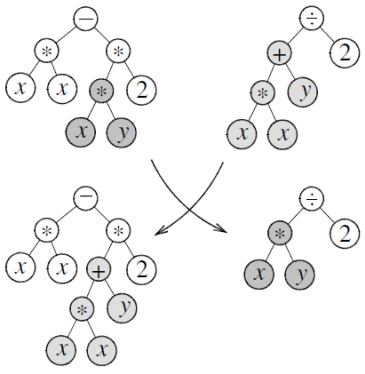
\includegraphics[scale=0.8]{Figures/crossover.png}
\caption{An example of a crossover between two individuals and their children as result}
\label{fig:cross}
\end{figure}

\begin{figure}[htp]
\centering
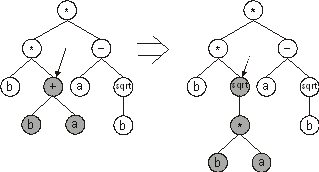
\includegraphics[scale=1.2]{Figures/mutation.png}
\caption{An example of a mutation applied to an individual}
\label{fig:mut}
\end{figure}

One of the problems with genetic programming is searching for the correct parameters to solve a specific problem. For each problem
a specified number of populations, generations needs to be provided e.g the percentage of the population to which crossover and
mutation are going to be applied. In more advanced cases the types of mutation and crossover algorithms need
to be specified. Another complication is choosing the correct fitness function to evaluate the correctness of the individuals. If 
an incorrect fitness function is defined an individual with seemingly good fitness value may be far from correct. The primitive
and terminal sets need to be wisely chosen as well. If too many primitives are chosen the generations might not be enough to 
find a solution to the problem because the search boundaries were expanded. However if small sets are chosen we are 
limiting the search boundaries or the individuals won't have a sufficient primitive set to satisfy the required functionality.
\paragraph{}
Using this methodology multiple problems can be solved. A common and a simple one is symbolic regression. In the case
of symbolic regression an individual represents a mathematical expression and is evaluated against another expression
specified in the fitness function. In this project this technique is uesed as a proof
of concept for the capabilities of the framework.

\section{What are Web Services?}
Web services are one of the main methods to provide utility computing. A definition for a web service is  
\begin{quote}A software system designed to support interoperable machine-to-machine interaction over a network. It has an interface described in a machine-processable format.\end{quote}
They represent an easy way for developers and clients to access and compute information. Usually through an API users are
being able to communicate with a web service although sometimes they need to be accessed with raw URL or HTTP request.
Unlike traditional client/server models, such as a Web server/Web page system, Web services do not provide the user with a GUI.
Web services instead share business logic, data and processes through a programmatic interface across a network. The applications
interface, not the users. Developers can then add the Web service to a GUI (such as a Web page or an executable program) to offer
specific functionality to users.
\paragraph{}
Web services hold many benefits for developers. They represent components on the web that can be plugged in any project
or software so it's functionality can be used. It improves communication between companies and users because information
is distributed much faster. A good example of a web service is of Google who provide an API to their GPS maps which when 
given longitude and latitude return a map with the location of the user. This service has improved the user experience
for many devices and because of it's good implementation has made the implementation of other similar services almost
obsolete.
\paragraph{}
A problem with web services are that if they go offline or they have a bug, they affect the whole network and every
user using them. Every non-open sourced framework is essentially a black box and the way it uses it's parameters is unknown.
However these problems are minor to the overall benefit of the web services. Because of the way the internet works
the amount of web services has essentially created a distributed system with multiple components. Developers can integrate
complex systems easier than before and can easily plug in additional functionality as long as the right web service is there 



\section{Aim}
The purpose of the project is to develop a framework that can clone a web service.
Theoretically it is possible to complete this through genetic programming. Initially the project
was separated into three steps - evaluate individuals over a network, clone and existing web service and improve a
web service. The project aims to clone an external web services and provide a GUI to
generate the configuration files needed for the framework to work.
\paragraph{}
Theoretically when using an external web service we know the parameters we are giving to it, we have an idea of the way it 
works and we know the results. Combining this knowledge meant it was possible to use an external web service as a fitness
function to our genetic program and a way to specify the primitive set used. After part two of the project
was completed it was proved that it is possible to clone the functionality of a web service. Because it is a proof of concept
project a simple web service was used in order to verify the expected result. However the project proves that with the right
choice of primitive set it is possible to clone the functionality of even more complex web services.

%==============================================================================
\chapter{Context}
A key part of the project was organization and project management. With a complex project like this there were many
factors and issues that needed to be considered before development could start. Research had to be done to identify
other similar projects such as \textit{Gen-o-fix: an embeddable framework for dynamic adaptive genetic improvement programming}.
Technologies had to be considered since multiple approaches to the implementation were available. Frequent meetings and 
iterations over requirements were key so the goals could be identified. Software development methods like agile development had to be used to help structure the
project, focus on the key goals and important features so sprints could be set up and development could be as efficient as possible.
\section{Related Work}
Before finalizing the idea of the project, research had to be done so previous related work can be found and compared. The project has a very
specific scope and there aren't many projects working towards a similar goal using genetic programming. The two of the projects were
\textit{Gen-o-fix: an embeddable framework for dynamic adaptive genetic improvement programming}[reference] and \textit{A Genetic Programming Approach to
Automated Software Repair}[reference].
\paragraph{}
\textit{Gen-o-fix}explores the concept of  genetic improvement programming (GIP) which goal is to automate software
maintenance. \textit{Gen-o-fix} is a GIP framework which allows a software system hosted on the Java Virtual Machine to be continually improved
(e.g. make better predictions; pass more regression tests; reduce power consumption). Initially \textit{Darwin} had the same goal but because of 
the complexity of the problem and the short amount of time it was decided to be left for future development. Similarly to \textit{Gen-o-fix},
\textit{Darwin} is also focused on creating a user-centric tool rather a research-centric one.
\paragraph{}
\textit{A Genetic Programming Approach to Automated Software Repair} is a project which idea is to repair bugs in off-the-shelf legacy C programs.
To achieve that the framework does three main modifications to the standard GP technique: (1) genetic operations are localized to the nodes along the execution path
of the negative test case; (2) high-level statements are represented as single nodes in the program tree; (3) genetic operators use existing
code in other parts of the program, so new code does not need to be invented. Initially \textit{Darwin} was supposed to include similar functionality
as well but it was again later excluded and kept for future development.
\paragraph{}
Both of the frameworks were focused on post-development processes like bug fixing, code improvement and code maintenance. These ideas are different
from \textit{Darwin}'s one of cloning web services however the concept for creating and modifying existing code through genetic programming is observed
in all three of the project. This made the papers a good source of information and approaches used for the development of \textit{Darwin}.

\section{Organization}
Frequent team meetings, proper software development method and good project management were key for the success of the project.
There were many unknowns in the beginning and as an inexperienced developer into the field of genetic
programming there were many basics that needed to be covered. Through this basics it was later possible to set the requirements,
sprints and organize a project around them.

\subsection{Agile Development}
As a development method agile development was chosen for the project. But in order to maintain a good project management a tool for
agile development was needed. Git hub \cite{github} was the version control used and PivotalTracker \cite{pivotal}
was the agile tool of choice.

\begin{figure}[htp]
\centering
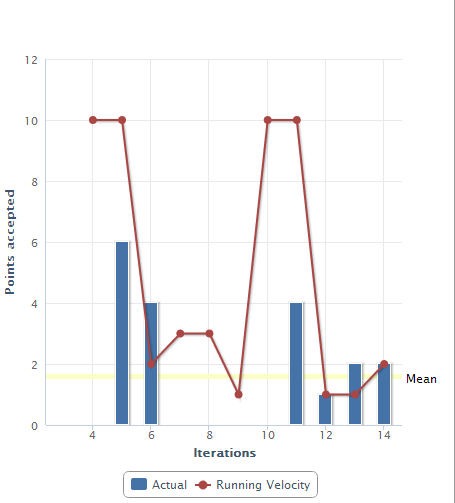
\includegraphics[scale=0.6]{Figures/pivotalGraph.png}
\caption{Velocity graph showing the sprints and the amount of work based on tickets completed in different iterations during first and second sprint}
\label{fig:pivotalGraph}
\end{figure}

PivotalTracker is a web based tool where all the development process was stored, place to put all the user stories, functional
and non-functional requirements, organize them and modify them easily. In the system it was easy to see when were the development bursts for the sprints and when was the post development time, when bugs were fixed, code was re-factored as seen in figure ~\ref{fig:pivotalGraph}.
This way the client can monitor how the actual development is going when was I working and on what feature. Pivotal tracker was used to monitor the progress
of the project as seen in figure ~\ref{fig:pivotalTracker}.

\begin{figure}[htp]
\centering
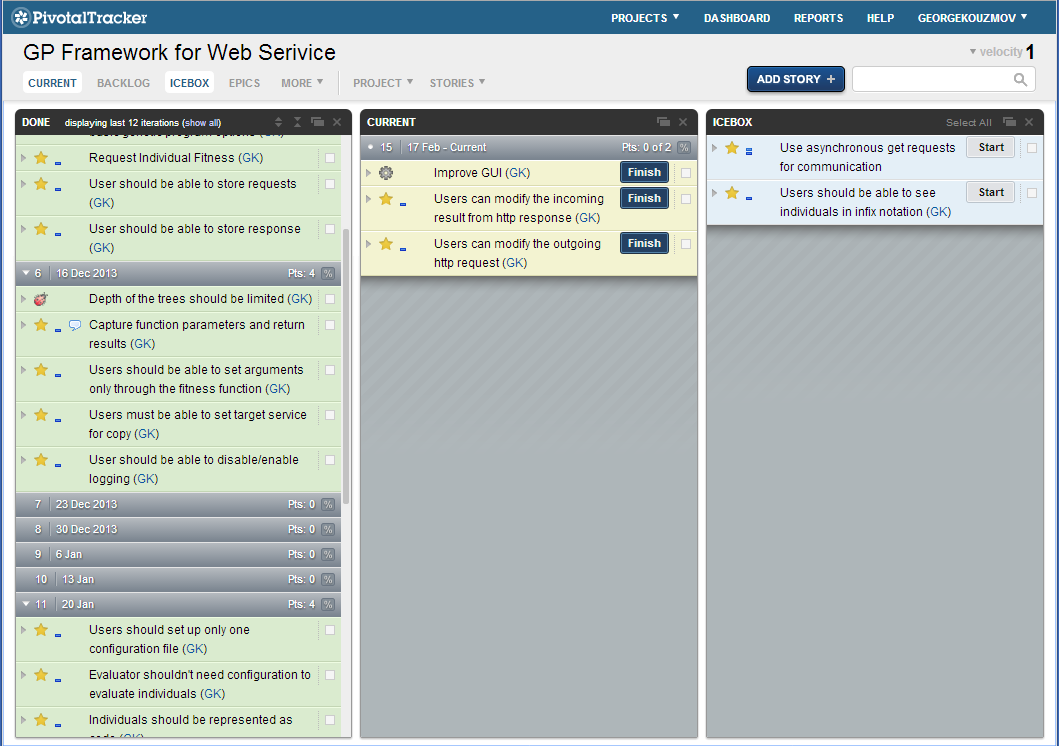
\includegraphics[scale=0.5]{Figures/pivotalTracker.png}
\caption{PivotalTracker and the way it is used by the project}
\label{fig:pivotalTracker}
\end{figure}

Git hub is the version control tool used for the project. Being a public code repository gave the opportunity to present the code easily to the client and
others as well. Frequent commits were done during the sprints. This way when the code broke during a sprint it could be reversed back to a working version.



\subsection{Requirements}
For requirements engineering an iterative approach was chosen. Through the first several meetings
different ideas and goals were considered until requirements were finalized. The MoSCoW\cite{moscow} method was used to
reach a common understanding with the client about the importance of each requirement and how
relevant it was to the project. MoSCoW method involves grading each requirement for how important it is for the project using the technique:
(M - must, C - could, S - should, W - won't).

\begin{table}[ht] 
\caption{Sprint one and sprint two of the framework} % title of Table 
\centering % used for centering table 
\begin{tabular}{l l} % centered columns (4 columns) 
\hline\hline %inserts double horizontal lines 
Sprint One – GP to create a web service & Sprint Two - GP to clone a web service \\ [0.5ex] % inserts table 
%heading 
\hline % inserts single horizontal line
1. Evolve a web service - M & 1. Integrate with DEAP - M \\
2. Fitness evaluation over REST - M & 2. Incorporate unit tests - C \\
3. Basic GP configuration - M & 3. Start from existing web service - S \\
4. Define function set - M & 4. Test through interpreter - S \\
5. Pre-set function set - S & 5. Use original web service as an "Oracle" - M \\
6. Generate python code of the best solution - M & - \\
7. Manipulate python code - S & - \\ [1ex]
\hline %inserts single line 
\end{tabular} 
\label{table:req} % is used to refer this table in the text 
\end{table}

However later on because of the project complexity and the time frame the third sprint was changed
from \textit{improving a web service} to creating a graphical user interface for easier configuration of the 
framework.  Even though requirements were set, small changes were done through out the development process
to suit the current situation and improve the software product. Requirements are displayed in table \ref{table:req}

\begin{table}[ht] 
\caption{Basic requirements for the project's technologies} % title of Table 
\centering % used for centering table 
\begin{tabular}{l} % centered columns (4 columns) 
\hline\hline %inserts double horizontal lines 
Basic Requirements \\ [0.5ex] % inserts table 
%heading 
\hline % inserts single horizontal line
1. Must be implemented in python \\
2. Must use a REST framework (CherryPy) \\
3. Develop or choose a genetic programming framework (DEAP) \\
\hline %inserts single line 
\end{tabular} 
\label{table:breq} % is used to refer this table in the text 
\end{table}

Before the requirements for each sprint were built there were basic requirements that needed to be identified as seen in table \ref{table:breq}. 
Framework for genetic programming and a REST framework had to be chosen. Weeks of research were dedicated to find the most suitable frameworks.
The only initial requirement was that the project should be done in python and later on after the client agreed with the technologies used they
were  added to the basic requirements. Knowing and understanding the technologies that would be the building blocks of the project helped guide 
the writing of the sprint requirements later on.


\subsection{User Stories and Sprints}
As mentioned before, the project is focusing on a user-centric tool. A list of user stories was created for the client
explaining the way he and any potential user was going to interact with the framework. The list
of stories was later iterated until there were set of user stories defining each of the sprints
as seen in figure \ref{table:userstories}.
\begin{table}[ht] 
\caption{Sprint one and sprint two of the framework} % title of Table 
\centering % used for centering table 
\begin{tabular}{l} % centered columns (4 columns) 
\hline\hline %inserts double horizontal lines 
Sprint One\\ [0.5ex] % inserts table 
%heading 
\hline % inserts single horizontal line
User should be able to disable/enable logging\\
User should set up only one configuration file\\
Users should be able to see individuals in infix notation\\
Users should be able to set arguments only through the fitness function \\

\hline\hline 
Sprint Two\\
\hline
User must be able to set target service to copy\\
User should be able to graph individuals\\
User should configure the framework through XML\\
\hline\hline 
Sprint Three\\
\hline
Users should chose from pre-set primitive functions\\
User should be able to generate XML file through a GUI\\
User should modify the incoming result from http response\\
User should modify the outgoing http request \\
\hline\hline 
\end{tabular} 
\label{table:userstories} % is used to refer this table in the text 
\end{table}

\begin{enumerate}
\item \textbf{Sprint One} was focused on evaluating individuals remotely
	\begin{enumerate}
	\item Configuration of basic genetic programming parameters.
	\item Create a class for defining and reading of primitive set.
	\item Converting DEAP individual to python code for easier evaluation.
	\item Create a base for cloning webservices.
	\end{enumerate}
\item \textbf{Sprint Two} was focused on cloning a web service.
	\begin{enumerate}
	\item Use existing web service as a fitness function.
	\item Automation of configuration.
	\item Use a single URL for selecting the target webservice.
	\end{enumerate}
\item \textbf{Sprint Three} aimed for creating a more interactive and easy way to configure the system.
	\begin{enumerate}
	\item Use of XML file to configure the framework.
	\item Create GUI for generating the XML file.
	\item Providing request and response handlers for handling communication with webservices.
	\end{enumerate}
\end{enumerate}


\subsection{Meetings and Minutes}
The core purpose of the meetings was to iterate through the development process with the
client. Initially it was only explanation of the project, genetic programming, possible
technologies and identify what can be developed for the time frame set for the project.
Every week since week two there has been a project meeting. They were helpful for me and 
for the client so we can clear the ideas that we had, form them into one and work towards
the same goal. The client's expertise in genetic programming and frequent meetings helped me 
understand how it works in little time so it was possible to begin development.
\begin{figure}[htp]
\centering
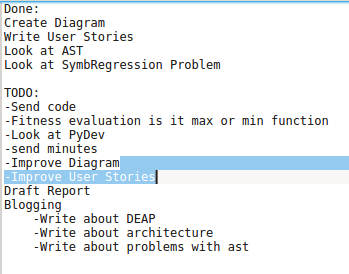
\includegraphics[scale=0.8]{Figures/minutes.png}
\caption{The minutes format and what was discussed in them}
\label{fig:minutes}
\end{figure}
Since day one minutes were introduced to follow the development of the project. This included reading
papers, learning concepts, testing technologies. Minutes became the main way of following
the project progress and a way for setting small goals for the week. Minutes also shaped
the meetings by being able to discuss step by step the goals set from previous time. Every
meeting had the same structure, it was discussed - what was done, what were the problems, 
new issues were addressed and possible solutions. The format of the minutes is shown
in figure \ref{fig:minutes}


%==============================================================================
\chapter{Design}
When designing the framework the key principle was to provide a simple way to control the key parameters in a genetic program.
The scope of the project is quite big and so is it's complexity so a key design feature was modularity. Component based software
engineering practices were used throughout the project, helping to organize the multiple technologies used.
\section{Multiple Technologies}
Among the key issues in the development was combining all the technologies used in the project.
\begin{itemize}
\item genetic programming framework
\item REST based web service
\item XML parser
\item GUI
\item code inspection
\item code generation
\end{itemize}
For each component there were multiple options available.
\subsection{RESTful Web Services} 
RESTful web services were needed for creating a service that can evaluate individuals over a network. Simplicity was important for the framework we are
choosing. WebPy\cite{webpy}, CherryPy\cite{cherrypy}, Flask\cite{flask}, Bottle\cite{bottle} and Django\cite{django} are commonly used frameworks. Each was compared as seen in figure \ref{fig:webtab} to identify the best candidate. 
However CherryPy and Django are the only frameworks that handle POST and GET request correctly, without any problems. In order to fix this issues with WebPy, Flask\cite{flask} or Bottle\cite{bottle} additional
libraries would have been needed. It was desired to avoid more dependencies because they would just make the project more complex. That meant the choice was between two. The more lightweight
choice was CherryPy but that wasn't the only reason why the project was chosen. A potential deployment platform was the Glasgow Raspberry Pi Cloud\cite{picloud}. Because CherryPy provided support for Raspberry Pi\cite{raspi} it was the obvious choice.

\begin{figure}[htp]
\centering
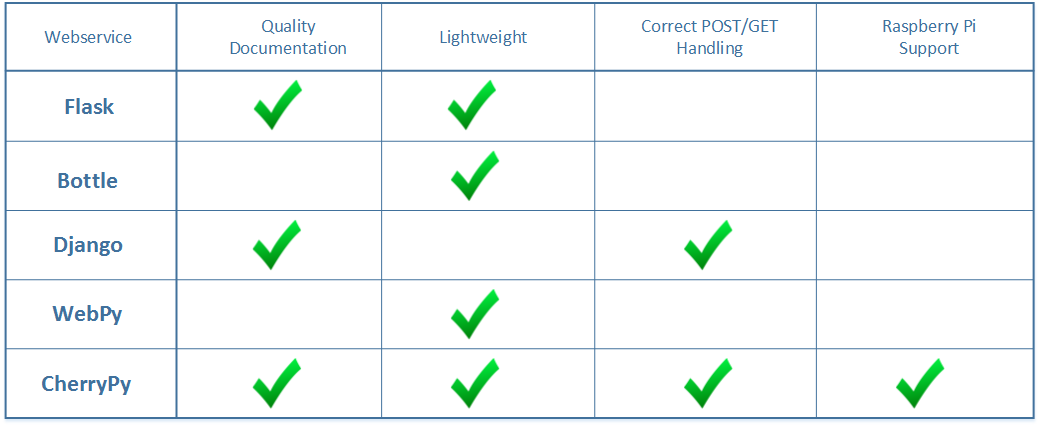
\includegraphics[scale=0.6]{Figures/webtable.png}
\caption{Comparison between five of the chosen webservices}
\label{fig:webtab}
\end{figure}

\paragraph{}
\textbf{CherryPy}
is a minimalistic python object-oriented framework which focuses on flexibility and has a reliable HTTP/1.1-complient, WSGI thread
pooled web server. It requires a small amount of source code to run it, making it very useful to take the purpose of the project. Darwin's webservice component
needs to be light in order to run either with multiple instances on a single server or run on a small devices like a Raspberry Pi.
\subsection{Genetic Programming Framework}
Genetic programming frameworks didn't have as many choices as RESTful web services however there was the option of implementing one.  Pyevolve\cite{pyevolve}, pystep\cite{pystep}, pygene\cite{pygene} and DEAP\cite{deap} were 
the only choices for genetic programming frameworks in python. None of them was minimalistic and simple enough, however implementing a genetic programming framework seemed a more complicated task
that could slow down the project and its final result. The most common and supported one was
the DEAP framework that also had really good documentation, tutorials and examples making it the correct choice. However as a future development option for the project
remains creating a genetic programming framework related to the project.
\subsection{Code Inspection and Generation}
Code inspection and generation was needed in order to achieve automation. Code inspection is used to extract source and information from live objects (e.g. modules, classes, methods, functions, tracebacks, 
frame objects, code objects). Generation is used to create new code objects and execute them in the scope of the program.
For inspecting code the best solution was the \textit{inspect} library which provided a way to extract source and other parameters from functions. It is a library that comes with python, 
has great documentation, examples and tutorials which proved positive for the speed of development.
\paragraph{}
Among one of the problems with using DEAP was it didn't support conversion between individuals and python source code or AST ( Abstract Syntax Tree). Representing an individual as raw code or an AST meant that 
the evaluating web service can be simplified even more. Using AST was very compatible with the way individuals are represented in genetic programming and it was more
robust and safe way of doing code generation rather than using raw string. However the more simple choice (raw strings), was selected due to pressure of time.  This suggested the idea of an open source contribution to the DEAP framework
 for generating python source 
and AST for a DEAP individuals.
\subsection{Graphical User Interface and XML}
Since the system is working with many parameters configuring them needed an abstraction. Using XML files for parsing parameters was the choice of abstraction. A parser was created
using lxml\cite{lxml} and connected with the graphical user interface.
Graphical user interface was the next step in project simplification. Its role was to generate XML files for the user with the ease of controlling all the parameters needed.
For creating GUI in python there are several good choices Tkinter, PyQT, wxPython. I've had prior experience with Tkinter and I wasn't excited about working with it again. It looked
much more complex compared to the other two. In sites such as StackOverflow the community was supporting wxPython. An additional benefit to using wxPython was the fact that there were a
lot of good tools for generating layout. However, my previous experience with GUI frameworks like Swing and its similarities with wxPython, gave me the advantage of understanding wxPython
quickly and writing a decent GUI in no time. In the end I didn't use any of the layout generating tools like wxGlade, wxDesigner or DialogBlocks because learning to use them was going to
cost almost the same time as learning wxPython.
\paragraph{}
\textbf{wxPython} follows the standard graphical library design pattern -MVC (Model View Controller).
This design is focused on separation of concerns making it perfect for building a GUI for creation of XML files. The model or the 
data is the configuration parameters used, the view is the wxPython's frame and interface and the controller is the XML parser making use of data.
The library provides an easy to understand and use API. The main component is a frame, each secondary component like a pane, button or a menubar
is added to it. The framework uses different types of sizers to organize the components in the frame. To create more complex layouts
sizers can be stacked. WxPython has a large number of pre-set and easy to configure dialogue boxes for almost any case that might be needed.
More complex components were later created because of framework's versatility and modularity.

\section{Architecture}
A top down approach was applied for identifying the major components in the system. Client's requirements were the starting point for identifying those components. They were
clear and simple enough to create a high level view of the framework , with which to explain the framework's basic behaviour and how it's going to work see figure ~\ref{fig:sprints}. 

\begin{figure}[htp]
\centering
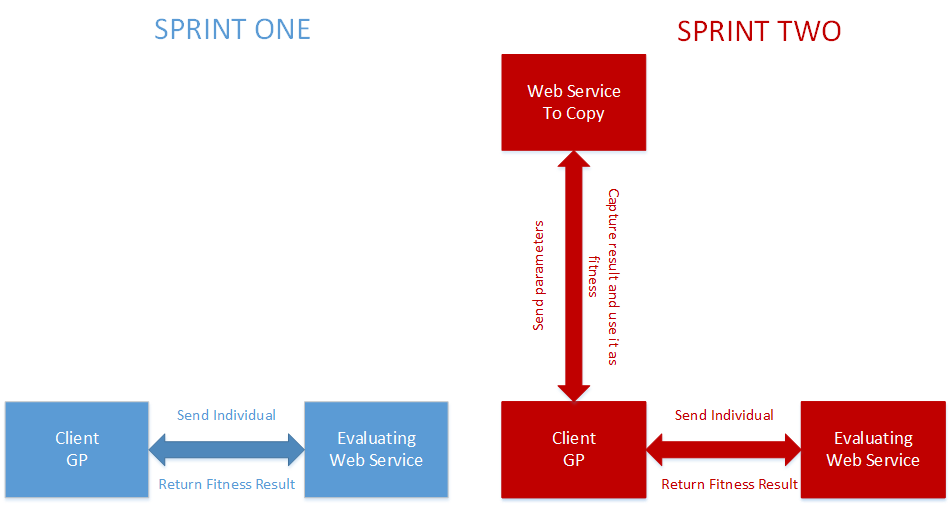
\includegraphics[scale=0.7]{Figures/sprints.png}
\caption{Top level view of sprint one and two}
\label{fig:sprints}
\end{figure}

By displaying the way the high level components communicate it was later possible to identify lower level ones.

\subsection{Overall Design}
After the high level components were designed, the user stories helped create a more detailed view of them. At that point of
time the project focused on sprint one which meant focusing on evaluating individuals over a network.
User stories helped identify how user was going to approach the framework hence it was able to create components with known
input and return parameters. The result was a high level view of first sprint with all of it's components identified see figure ~\ref{fig:firstSprint}

\begin{figure}[htp]
\centering
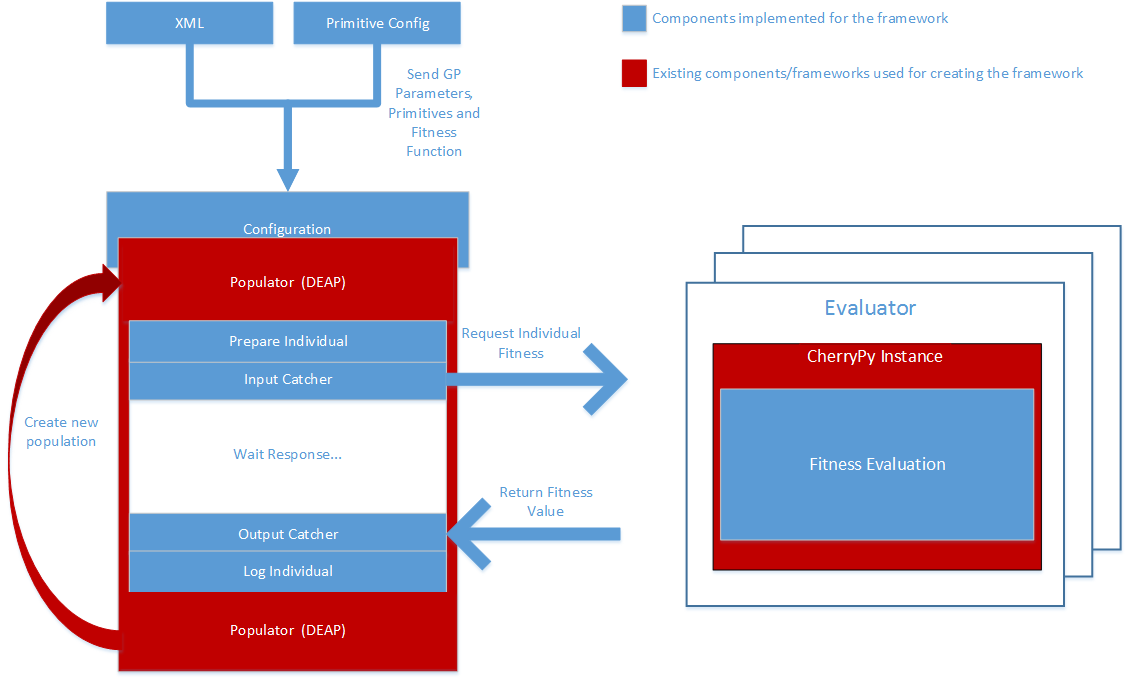
\includegraphics[scale=0.6]{Figures/FirstSprint.png}
\caption{High level view of sprint one and the identified components used}
\label{fig:firstSprint}
\end{figure}

Even though python2.7 unlike python3.3 is a semi object language for better use of software engineering practices and better ordering of the project,
objects were used to represent the different components. The diverse capabilities of python and large set of libraries helped design a complex framework with very simple architecture. Later on more 
specifics for the client design will be explained. As you can see in figure ~\ref{fig:firstSprint} Configuration, Configure Genetic Program and Genetic Program represent the three main components of the client and
CherryPy with an evaluation component represents the evaluating web service. This design helped us insert the technologies we are using at the correct
places. For example Input Catcher and Output Catcher were later on substituted by a single component that using the requests library handles the requests
and logs the traffic to the evaluator. These steps from top to down helped us clearly identified the classes that are going to be in the components.

\subsection{Client}
Before explaining how the client works, the DEAP framework needs to be explained. It is configured through a set of method calls
to a \textit{toolbox}; this \textit{toolbox} is prior configured by a \textit{primitive set} where all the primitives and 
terminals that the genetic program is going to use are defined. The toolbox give easy API for accessing and controlling the individuals,
generations and population as well as methods that invoke mutation, crossover and evaluation over the population.
\paragraph{}
Knowing how the DEAP framework works, it was later obvious that the same parameters needed for DEAP's configuration
were going to be needed for Darwin's as well. Through the \textit{PrimitiveConfig} class shown in figure ~\ref{fig:classd}
it was possible to set all the primitive functions and the fitness function needed for the program. Later on the client decided
that there should be a pre-set number of primitives and the user would choose through the GUI which to enable. However in
the case of an advanced user if additional primitives need to be added the class can simply be extended and add them as
normal methods. No other configurations regarding the primitives need to be done since Darwin is handling everything else.

\paragraph{}
In figure ~\ref{fig:classd} you can see that for the configuration of the genetic programming algorithm other parameters are needed which
are not specified in the \textit{PrimitiveSet} class; this is done in the \textit{Configuration} component. When setting up the framework they can be set manually or configured
by an XML file that carries all the information needed. There are only two parameters that are mandatory and the framework
won't work without them - the address of the evaluating web service and the target service that needs to be cloned. Any other
parameter is automatically set up with a standard value for solving the symbolic regression problem. The class that configures
the framework acts like a data model since all the parameters needed through any other step of the framework is instantiated there.
This data model is later used by the \textit{Populator} component.
\paragraph{}
The \textit{Populator} class is basically a wrapper around the DEAP framework. The class creates the first generation by
randomly generating individuals. Each individual is send over the network to the evaluating webservice. The evaluating webservice measures the fitness
of an individual and returns it. After each individual's fitness value is updated it
repeats the process until the number of generations are reached or an individual with 0.0 fitness is found. Besides executing the actual genetic program the \textit(Populator)
logs the traffic between the services and handles the output of the genetic program - either displaying the best individual or 
generating a web service working with the best individual.



\subsection{Evaluator}
The final big component is the \textit{Evaluator} \ref{fig:firstSprint}. It is a CherryPy service that can be executed on any machine running python and
 has only one method - evaluate. It would receive an individual, compare it to results from the target return fitness as a result. Initially design involved using DEAP individuals.
However evaluate it the same DEAP configuration needed to be set up on the evaluating side as on the client one.
This was impractical,slower, it was introducing many dependencies. The Evaluator needs
to be easy to set up, easy to modify because it is expected to be ran on multiple machines including Raspberry Pi.
Because of that individuals were later represented as source code which meant it was able to run on any machine
that runs Python. This way simplicity was achieved for this component by moving most of the overhead work to the client.


\section{GUI Design and XML}
A graphical user interface for generating the XML configuration file had to be designed for the third sprint.
Ease of configuration had to be provided for configuring the multiple parameters the framework provides . Because
it's a framework software project GUI is not as important as the more algorithmic parts of the project, but usability
and simplicity are design aims of the project.

\subsection{XML Configuration}
The XML file that is parsed between the GUI and the framework needed to be readable and editable by users. That meant that the
markup used had to follow standard design so it can be modified by users.
This designed provided a backup plan in case GUI implementation failed. However the GUI was created
which meant a parser needed to be implemented which was done with the help of \textit{lxml} library.

\subsection{Purpose of the GUI and Iterations}
While iterating through design decisions the idea was to make the GUI as familiar as possible. In many dialogues
and popular graphical user interfaces a similar layout is encountered - menubar on top, left to right and
top to bottom reading, bottom right buttons for completing the task see figure \ref{fig:guiex}. Because
of its purpose and the way its used the GUI looks more as a dialogue window - simple window that helps 
generate a file/configuration and its used for a short amount of time.

\begin{figure}[htp]
\centering
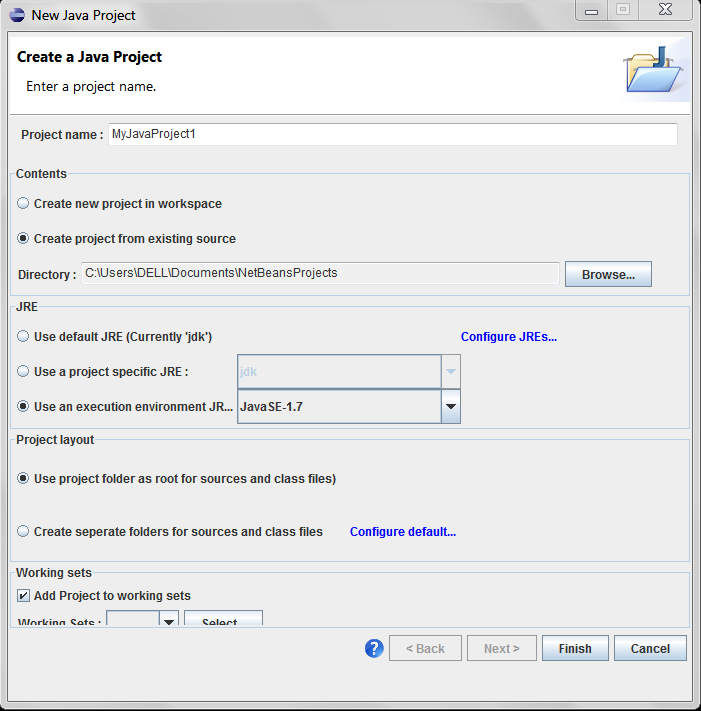
\includegraphics[scale=0.6]{Figures/gui_example1.png}
\caption{Example of a dialogue used for configuration of projects used in Eclipse editor}
\label{fig:guiex}
\end{figure}

The most important parameters - target IP address and client IP address,
are located at the top left corner of the window. Other parameters text fields are located from left  to right top to bottom
based on their relevance. That's why bottom left is located the button for generating the XML configuration
file hence finishing the process.

\begin{figure}[htp]
\centering
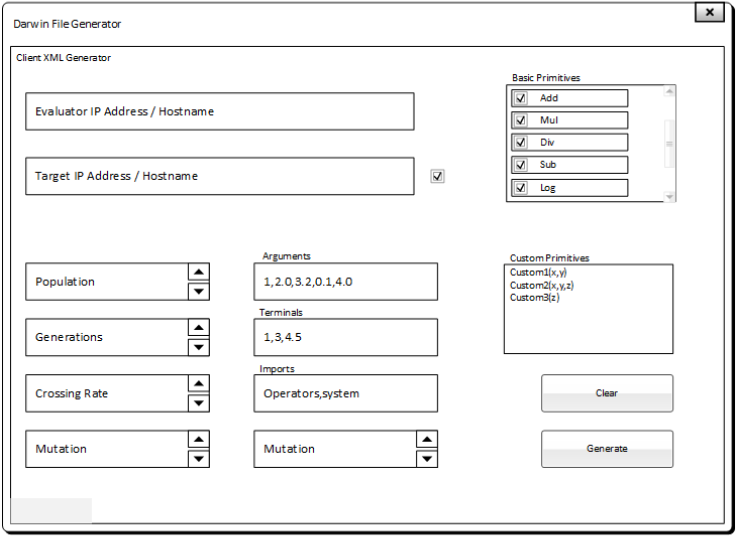
\includegraphics[scale=0.6]{Figures/guiit.png}
\caption{One of the iterations of the GUI showing all the possible parameters}
\label{fig:guiit}
\end{figure}

In the first iteration of the design additional features like adding custom primitives and selecting imports
for those custom primitives were added as you can see in figure \ref{fig:guiit}. However after discussion with the client it was later
decided that these features are part of the more advanced functionality of the framework. It was unnecessary to implement them in the GUI
 since they were available in the code where they would be 
normally reached and modified from a more experienced users that would use this functionality. The final iteration of the GUI design
 looked as displayed in figure \ref{fig:guiit}
 it


%==============================================================================
\chapter{Implementation}
During the first months of the project a lot of time was spend developing small components and testing
the technologies. This created the base for productive sprints. There were difficulties in the implementation
however the time spent testing out the technologies proved very useful in solving the problems quickly. The agile
development proved very successful for implementing step by step the functionalities of the project. Following
the architecture design strictly helped when modifications of components were done. 

\section{Use of Technologies}

\subsection{DEAP}
DEAP (Distributed Evolutionary Algorithms in Python) is a framework that supports both genetic algorithms and genetic programming.
It seeks to make algorithms explicit and data structures transparent. Hence making genetic programming easy by providing an easy way for primitives
to be created and access to crossover and mutation algorithms. Each of its features can be fine tuned through multiple parameters.
\paragraph{}
Similar to Darwin, DEAP emphasizes on loose coupling in its design, it uses multiple components that provide the necessary functionality
for the framework. The \textit{pset} is a class through which all the configuration related to the primitive set is done. Primitives are defined
through mapping any defined function or method and declaring the amount of arguments they are taking. In addition the terminals are defined where
there is a pre-set of constants that can be utilized. Arguments for the genetic program are also defined in through the \textit{pset} hence 
separating it from other components so it can be extracted and manipulated individually.
\paragraph{}
Another core component of the DEAP framework is the \textit{toolbox}. This is the component where the genetic programming is configured. Parameters
like maximum depth of an individuals are specified as well as the algorithms for crossover and mutation. The framework gives the flexibility to define your
own mutation and crossover algorithms as well as manipulate their rates and the size of the population and generation. Fitness function is specified in the toolbox 
and later maps to the toolbox. After configuration of the primitive set and the genetic
programming parameters is done the population is generated. There is an automatic way of doing it through special DEAP functions however for Darwin
a more complex approach was chosen which will be later explained. The statistics module takes the generations and creates
set of statistics that can be displayed ( e.g. mean of a generation, best and worst individual ).



\subsection{Requests}
Requests is a simple python library that provides easy API for sending HTTP requests and receive responses. It is an
abstraction over the standard python library \textit{urllib2}. Requests library works by creating a requests object
which is filled in with the data it needs - URL as string, parameters in the form of dictionary. This object has methods like \textit{get} and \textit{post}
which send respectively GET or POST request to the target URL with the parameters. The \textit{get} and \textit{post} method return a
response object that contains the result in text format which in the case of web services is normally XML.

\section{Core Components and Functionality}

\subsection{DEAP Set Up}
DEAP is used in Darwin framework by utilizing the loose coupling used in its design. Each of the DEAP components is configured
separately. This way the processes of Darwin framework that are dependant on DEAP can be split into multiple functions so loose coupling can
be achieved.
\paragraph{}
The \textit{Configuration} class as seen in figure \ref{lst:config} consists of the \textit{pset} and \textit{toolbox} components
from the DEAP framework. In order to set the needed information for the genetic programming an abstraction layer is added to the DEAP framework.
Because the purpose of Darwin is known - solve symbolic regression problems, there are many pre-set parameters used in the configuration, hence there are 
fewer parameters to be specified for Darwin. This level of abstraction both simplifies the use of the
framework by lowering the amount of parameters needed and creates a link between Darwin and DEAP. \textit{Configuration} provides a \textit{configure()} method
that organizes the Darwin variables and sets up the DEAP framework underneath. This \textit{configure()} method does four things as seen in \ref{fig:classdi}:

\begin{enumerate}
  \item \textit{setPrimitiveFunctions()} extracts the primitive functions from the user defined class that extends \textit{PrimitiveConfig} . It takes an instance
of each of the methods and maps them to the DEAP framework.
  \item \textit{setTerminals()} gathers a list of all defined terminals and instantiates them in the DEAP framework.
  \item \textit{configureToolbox()} is a more complex method where DEAP's \textit{toolbox} is configured:
  \begin{enumerate}
	\item Creates an individual by specifying the type of structure it is going to use (PrimitiveTree in the case). 
	\item Checks if the individual is aiming for minimum or maximum fitness function; this sets the individual to either look for lowest or 0 fitness value or the maximum among individuals.
	\item Defines the initial size of the individuals, the size of the population and generation based on the user parameters.
	\item Maps all the mutation and crossover methods to pre-defined DEAP algorithms which are good for the purpose of the genetic program.
	\item Since DEAP uses decorators to modify the generated individuals, decorators need to be defined to limit the size of an individual.
  \end{enumerate}
  \item \textit{configureArgumetns()} takes the test arguments given by the user and based on their names maps them to DEAP so the individuals can take arguments.
\end{enumerate}

\begin{landscape}
\begin{figure}[htp]
\centering
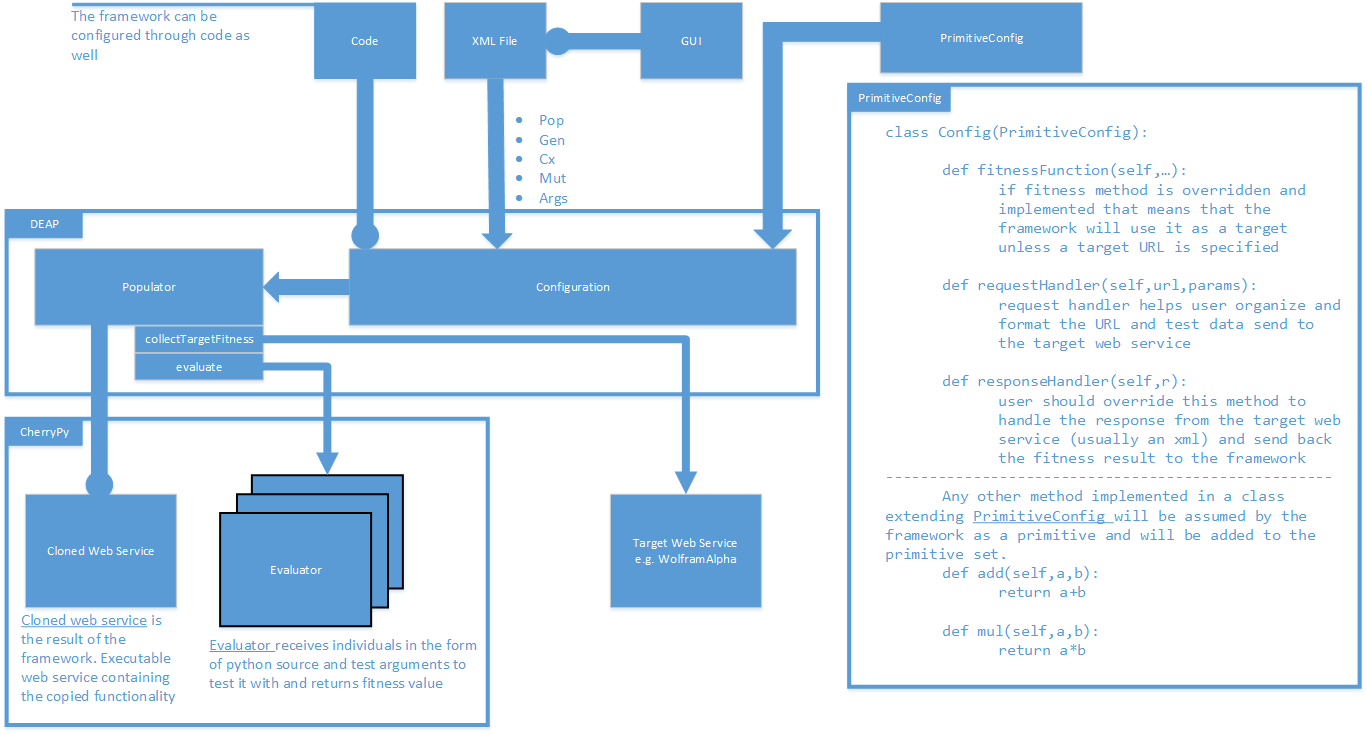
\includegraphics[scale=0.7]{Figures/Class.png}
\caption{Lower level component diagram showing the functionality and usage of each class/component (this is a copy for easier readability}
\label{fig:classdi}
\end{figure}
\end{landscape}

\begin{landscape}
\begin{lstlisting}[language=Python,caption={The core method in Configuration class that configures the DEAP framework},label={lst:config}]

def configureToolbox(self):
    if not self.isMax   : creator.create("FitnessMin", base.Fitness, weights=(-1.0,))
    else                : creator.create("FitnessMax", base.Fitness, weights=(-1.0,))

    creator.create("Individual", gp.PrimitiveTree, fitness=creator.FitnessMin, pset=self.pset)
    self.toolbox.register("expr", gp.genRamped, pset= self.pset, min_=self.depthInitialMin, max_=self.depthInitialMax)
    self.toolbox.register("individual", tools.initIterate, creator.Individual,  self.toolbox.expr)
    self.toolbox.register("population", tools.initRepeat, list,  self.toolbox.individual)
    self.toolbox.register("select", tools.selTournament, tournsize=3)
    self.toolbox.register("mate", gp.cxOnePoint)
    self.toolbox.register("expr_mut", gp.genFull, min_=0, max_=2)
    self.toolbox.register('mutate', gp.mutUniform, expr= self.toolbox.expr_mut)

	self.toolbox.decorate('mutate',gp.staticDepthLimit(self.maxDepthLimit))
    self.toolbox.decorate('mate',gp.staticDepthLimit(self.maxDepthLimit))
\end{lstlisting}
\end{landscape}	

\subsection{Generation of Individuals}
Individuals are created and generated in the \textit{Populator} class. It is a component of the framework where
the genetic programming is done and handles output. It also contains functionality for communicating with other
web services, either an evaluator or a target web service for cloning.
\paragraph{}
Unlike the \textit{Configuration} class the \textit{Populator} doesn't work with the \textit{pset} and \textit{toolbox} DEAP
components directly. It uses them to generate individuals and apply a mutation or crossover algorithm to it. Instead of using
the standard genetic programming algorithm that DEAP provides by calling a single function, the algorithm had to be implemented 
manually. As seen in \ref{lst:populate} the offspring is initialized by copying it from the initial population. This first population is a
generation of random individuals with depth between 1 and 3. 

\begin{lstlisting}[language=Python,caption={Populate function responsible for generating individuals},label={lst:populate},breaklines=true]

 def populate(self):
    for gen in range(self.configuration.gen):
        self.offspring = self.toolbox.select(self.population, len(self.population))
        self.offspring = map(self.toolbox.clone, self.offspring)
        self.crossover()
        self.mutation()
        invalid_ind = self.nonEvaluated(self.offspring)
        fitnesses = self.toolbox.map(self.evaluate, invalid_ind)
        for ind, fit in zip(invalid_ind, fitnesses):
            ind.fitness.values = fit
        self.population = self.offspring
        self.hof.update(self.population)

    self.outputIndividuals()
\end{lstlisting}

To each generation crossover and mutation functions are applied. However both of the functions are modified so each
individual is evaluated separately. The whole avoiding of DEAP's standard genetic programming function is because evaluation
is not done in the \textit{Populator} but by the \textit{Evaluator}. In order to make use of the decorators the crossover
and mutation function a manual substitution of the generation is done as seen in \ref{lst:populate}.

\begin{lstlisting}[language=Python,caption={Modified mutation method to substitute each parent with its children},label={lst:populate}]

def mutation(self):
    for i in range(len(self.offspring)):
        if random.random() < self.configuration.mut:
            self.offspring[i], = self.toolbox.mutate(self.offspring[i])
            del self.offspring[i].fitness.values
\end{lstlisting}

\subsection{Evaluation Over a Network}
Evaluation over the network is done using the requests python library creating HTTP requests to the \textit{Evaluator} web service that is created using the CherryPy framework.
\paragraph{}
If no target function is specified and a target web service is, then the requests library is used to send the test arguments to the web service so it can get the correct result. This result
is put with every set of test arguments in a dictionary and sent to the evaluator together with an individual. Initially the idea was to have multiple evaluators processing the
individuals which meant making asynchronous requests to multiple web services. However the complexity of the task was too high and the development time for such a component would
of been too long, so only a single evaluator is used.
\paragraph{}
The easy parsing of parameters in CherryPy made it comfortable to send individuals as parameters to the web service and their test arguments so they can be evaluated. Initially
the web service had to set up additional DEAP configuration in order to evaluate an individual and return the result. However there was a lot of complexity and dependencies were
too many and so it was later re-factored to parse the source code of an individual to the \textit{Evaluator}. This simplifies of the evaluator to 
a single simple method.

\begin{lstlisting}[language=Python,caption={The soruce of the evaluator},label={lst:evaluator}]
class BaseCherryPy:

    def evaluate(self,individual,arguments):
        arguments = eval(arguments)
        diff=0
        for i in arguments:
            sys.argv = i[0]
            with stdoutIO() as s:
                exec(individual) in {}
            try:
                res = float(s.getvalue())
                diff += (res - i[1])**2
            except:
                diff = sys.float_info.max
        return str(diff)

    evaluate.exposed=True
\end{lstlisting}

In order to run the evaluator the class that is used by CherryPy needs to be either \textit{BaseCherryPy} or a class extending it. What \textit{BaseCherryPy} contains
is a method that has the exposed flag set to true that handles the sent individual. The client is always calling the method called \textit{evaluator} see \ref{lst:evaluator} with two parameters.
One is an individual in Python source code and the second is a dictionary with test arguments and compare values from the target. What the method does is it sets the system arguments
of the python interpreter to the test arguments and after that executes the source code in a different context. Then by overwriting the \textit{contextmanager}\footnote{Note that the overwriting of contextmanager
wasn't done by me but the stackoverflow user isedev in the thread http://stackoverflow.com/questions/14708216/showing-current-output-from-exec-in-python handling this issue} the python standard output is
redirected back to the original context ( the one of the evaluator).


\subsection{Code Generation}
Code generation is the main technique for automation used in Darwin framework. It uses
the inspect library to gather the data and code needed for code generation. The main methods
for extraction of code are located in \textit{PrimitiveConfig}. The methods that use the inspect library
are extracting the code of the functions chosen as primitives as seen in fig \ref{lst:inspect}.
The method \textit{functionArgs} extracts the arguments hence the signature from target primitive function
given its name.

\begin{lstlisting}[language=Python,caption={Function extracting the arguments of a primitive based on its name},label={lst:inspect}]
def functionArgs(self,funcName):
    func = getattr(self,funcName)
    args = inspect.getargspec(func)[0]
    del args[0] # removes 'self'
    return args
\end{lstlisting}

The method for converting DEAP individual into source is located in PrimitiveConfig as well. In the \textit{helper} module
there are multiple functions constructing different parts of the individual source as seen in figure \ref{lst:gen}.

\begin{lstlisting}[language=Python,caption={Function in PrimitiveConfig class that gathers source code parts of the individual},label={lst:gen}]

def getSource(self, imports,individual,arguments):
    source = generateImports(imports)
    source+= generateFunctions(self,False)
    source += generateMain(arguments,individual,False)
    source += "print main(**sys.argv)\n"
    return source
\end{lstlisting}

The \textit{getSource} method collects source from three main methods located in the \textit{helper} module.

\begin{enumerate}
\item \textit{generateImports} based on a list of module names is generating the import statements.

\item \textit{generateFunctions} extracts the source and the signature of a primitive by removing the self argument in the method. 
\item \textit{generateMain} creates a main function that accepts as parameters the arguments of an individual. Later the DEAP
individual that is represented as a stack of functions is executed through a lambda expression that yields the result
\item the main method is called using system arguments as a dictionary. The result is printed to the standard output
so it can be forwarded to the original context when executed
\end{enumerate}

The same methods are used when generating a webservice as seen in figure \ref{lst:webs}. The difference is the code is wrapped into a class that is used
by CherryPy meaning the primitive signature and the lambda expression need to include the \textit{self} notation. The webservice has
an index method that is called only by accessing the URL that returns the result of the individual.

\begin{lstlisting}[language=Python,caption={A generated web service that is the result of the Darwin framework},label={lst:webs}]

class ClonedWebService(BaseCherryPy):

    def mul(self,a,b):
        return operator.mul(a,b)

    def main(self,r):
        r = float(r)
        ind = lambda r: self.mul(self.mul(3.14, r), r)
        return ind(r)

    def index(self,r):
        return self.main(r)
    index.exposed = True

cherrypy.quickstart(ClonedWebService())
\end{lstlisting}

\subsection{GUI}
For python GUI development wxPython was a great choice because it offered simplicity and progress was easy.
The framework supports loose coupling and high cohesion, it gives the opportunity to develop separate components
and combine them later. This design feature was used to develop a component for each set of elements in the
wireframe. Later on it was decided that advanced functionality should be opt out from the GUI and only
basic configuration should be available. The result was the following GUI \ref{fig:guiimp}

\begin{figure}[htp]
\centering
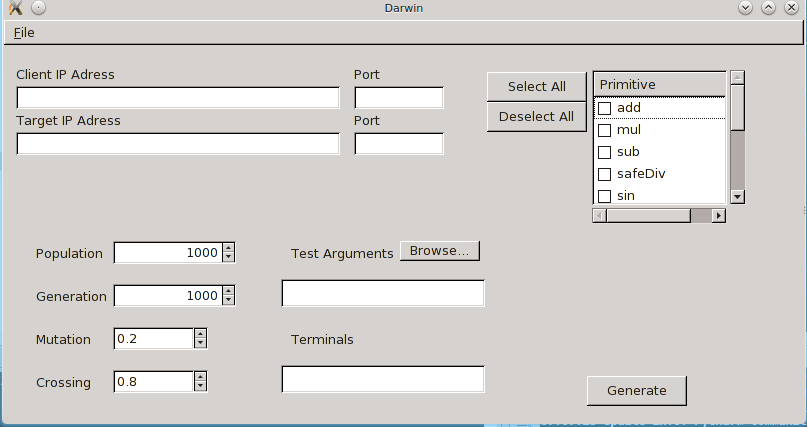
\includegraphics[scale=0.7]{Figures/gui.png}
\caption{Graphical user interface for the Darwin framework that generates XML files}
\label{fig:guiimp}
\end{figure}

The GUI was split into five components \ref{lst:guicode}.

\begin{enumerate}
	\item \textit{InitMenu()} initializes the menubar on top, creates each of the menu and sub-menu options and 
	handles the functionality of the menu items.
	\item \textit{InitTexts()} creates a pane that has text input fields for the URLs of the target web service and 
	the evaluator.
	\item \textit{InitAttributes()} returns a pane that has fields that specify the parameters used in the genetic program (e.g. crossing rate, mutation rate, population size, number of generations)
	\item \textit{InitPrimitives()} creates a primitives selector. The selector is created by combining several wxPython components like \textit{scrollable panes}, \textit{CheckListControl} and multiple
	sizers to organize the buttons and create a better feel.
	\item \textit{InitButtons()} simply creates a plane with the button \textit{Generate} however it would be expected that later on more buttons would be added
\end{enumerate} 

\begin{lstlisting}[language=Python,caption={The method in the GUI that initializes all the components used},label={lst:guicode}]
def InitUI(self):
    self.InitMenu()
    textPanel = self.InitTexts()
    attrPanel = self.InitAttributes()
    primPanel = self.InitPrimitives()
    buttPanel = self.InitButtons()
\end{lstlisting}

When the \textit{Generate} button is pressed the GUI is organizing all the data from the fields into a dictionary which is passed to the XML parser to generate the XML configuration file see listing \ref{lst:xmlf}

\begin{lstlisting}[language=XML,caption={XML file used by the framework for configuring the needed parameters},label={lst:xmlf}]
<config>
  <mut>0.2</mut>
  <arguments>
    <arg name="r" number="0">1</arg>
    <arg name="r" number="1">0</arg>
    <arg name="r" number="2">1.5</arg>
    <arg name="r" number="3">5</arg>
    <arg name="r" number="4">15</arg>
    <arg name="r" number="5">13.4</arg>
    <arg name="r" number="6">20.1</arg>
    <arg name="r" number="7">132.2</arg>
  </arguments>
  <pop>300</pop>
  <terminals>
    <terminal>3.14</terminal>
  </terminals>
  <cx>0.8</cx>
  <copyUrl>http://api.wolframalpha.com/v2/query</copyUrl>
  <basicPrimitives>
    <primitive>mul</primitive>
    <primitive>pow</primitive>
  </basicPrimitives>
  <evalUrl>http://localhost:8844</evalUrl>
  <gen>300</gen>
</config>
\end{lstlisting}



%==============================================================================
\chapter{Evaluation}
Evaluation is an important part of system development. \textit{Darwin} being a complex framework, extensive
tests needed to be ran over each of its components. Unit tests were used to verify the functionality of the
core components, system testing was used to evaluate the overall functionality and stability of the system.
User evaluation was used to test the usability of the framework and the graphical user interface.
\section{Unit Testing}
By separating the framework into several base components it was easier to split each of the components into
its core functions and apply unit tests to verify their correctness. However due to the complexity and
dependencies in the framework, test writing was complicated. Many of the functions depended either on 
the DEAP toolbox or on the primitive set which was responsible for generating DEAP individuals. They couldn't
be reproduced manually for the tests, so multiple components had to be enabled in order to verify the unit tests.
Since DEAP was an external framework with a stable release it was assumed that it is functioning correctly so no 
unit tests were ran on it specifically however components using it were extensively tested. Each of the components
had testing aims however not all functions were covered since their complexity or dependency was too high, thats why
they were left for system testing later on. This was the unit testing strategy:

\begin{enumerate}
  \item Unit tests on each of PrimitiveConfig's methods
  \begin{enumerate}
	\item Test pre-set primitives
	\item Test code generation
	\item Test utility functions
  \end{enumerate}  
  \item Test all of Populator's methods without the configuration methods or the more complicated ones which would be part of the system testing.
  \begin{enumerate}
	\item Test methods related to individual manipulation
	\item Test code generation
	\item Test fitness gathering functions 
  \end{enumerate}  
  \item Handle all the functions in the helper module excluding Proxy class that is going to be aprt of the system testing.
  \begin{enumerate}
	\item Test utility functions
	\item Test code generation
  \end{enumerate} 
\end{enumerate}

Through the unit tests many errors in the code generation functions were found so they had to be re factored. The imports used for the custom primitive set
weren't working properly so they had to be fixed. After the unit tests were created initially they were used for verification of code correctness after
a change in the code. If the unit test didn't work that meant there was an error in the code.
\paragraph{}
Among the bugs found through unit tests was a code generation one. The python source was missing the imports specified by the user. When a simple system
test was ran it couldn't be identified since the primitives used didn't include any external imports. However because of the modified configuration used
for unit testing the bug was identified on time.
\paragraph{}
Another problem was with the pre-set primitives. Because of the mathematical nature of primitives division by 0 had to be avoided.
In the simple system tests there were no examples with division by 0, the bug wasn't found until unit tests
for each primitive were executed.
\section{System Testing}
There were many dependencies in the framework, which made testing a very difficult task. So instead of spending
a lot of time trying to write complicated unit tests for each function/method in the code it was
decided it's easier to do system testing. In the case of methods like \textit{evaluate} where individuals were send to the evaluating
web service unit tests weren't an option because in order to test them individuals had to be generated manually. Generating
individuals was easy but generating the same ones every time so the test data can be robust was a problem. That's why after
other framework functionalities were verified system testing was done to prove the correctness of the more complex components.
\paragraph{}
For system testing the goal was to use a generated web service for cloning and a real world one. The first step of the system
testing was easy and simple enough. Testing proved successful and useful results were pulled out of it. For example a bug was
detected in which DEAP individuals were generated with depth above 90. This meant that the python stack was breaking and couldn't
evaluate the individual properly. The bug was fixed by modifying the way DEAP's decorator methods were used in the individual
generation. This helped clear a major issue and second stage of system testing could being. In the second stage Wolfram Alpha[ref] 
was used as an external web service targeted for cloning. The first issues was the way Wolfram Alpha was receiving parameters and
the responses in XML format. Since the framework didn't have functionality to handle the issue system testing was stopped and development
over request and response handlers was started. After completion of the tasks system testing was initiated again. Framework passed through
first and second stage of system testing. Second stage was tested with Wolfram Alpha. The framework succeeded to generate a web service that had the same functionality
as the expression used as input for Wolfram Alpha. The mathematical formula used was measuring the face of a circle. It was a formula
that was simple enough so cloning time can be short but complex enough to show the frameworks functionality.

\section{UI and Usability Testing}
An important feature for a framework is acceptance testing. Participants were used to evaluate the quality of the framework and check if the goals
to create an easy to use and simple framework were achieved. The participants were presented with tutorial for the framework, 
each of them had to have basic knowledge in programming. The choice of first to fourth year students presented a good study group since it presented people
with different levels of programming experience. The participants had to asses the quality of the 
tutorial, understanding of the framework and usability of the GUI. Each had to answer the following questions\cite{monkey}:

\begin{enumerate}
\item How helpful was it to understand the basics of the framework?
\item How complex it was to create the first examples?
\item How complex was to create the advanced example?
\item How far on the tutorial did you reach in 30 minutes?
\end{enumerate}
 
Second part of the evaluation participants had to asses the graphical user interface by answering the following questions: 

\begin{enumerate}
\item How intuitive is it?
\item How simple is it?
\item Were there enough options presented?
\item Can you give additional feedback that can help improve the GUI?
\end{enumerate}

In addition through the evaluation the participants were observed and notes based on their actions were taken to compare with their feedback. This way a more
accurate conclusions could be drawn. SurveyMonkey was used for the survey. Through the evaluation the following problems in the GUI and the tutorial were identified and fixed:

\textbf{Graphical User Interface}
\begin{itemize}
\item Omitting \textit{http} should still create a valid URL.
\item If no arguments are provided an error message should pop up
\item There should be help text for the \textit{terminals} field to specify it's format.
\end{itemize}

\textbf{Tutorial}
\begin{itemize}
\item There should be a link to the libraries/frameworks websites?
\item The version of each library/framework should be specified?
\item There should be more frequent code examples?
\end{itemize}

As seen in the results from the survey, participants had hard time with running the first example as seen in fig \ref{fig:firstex}. This was due to the multiple dependencies of the
framework, lack of installation script and ambiguity in the tutorial. However
in the end of the tutorial there was a high number participants that understood the basic framework functionality. Most of the participants managed to complete the tutorial
in less than 30 minutes, however these 30 minutes didn't include set up time.

\begin{figure}[htp]
\centering
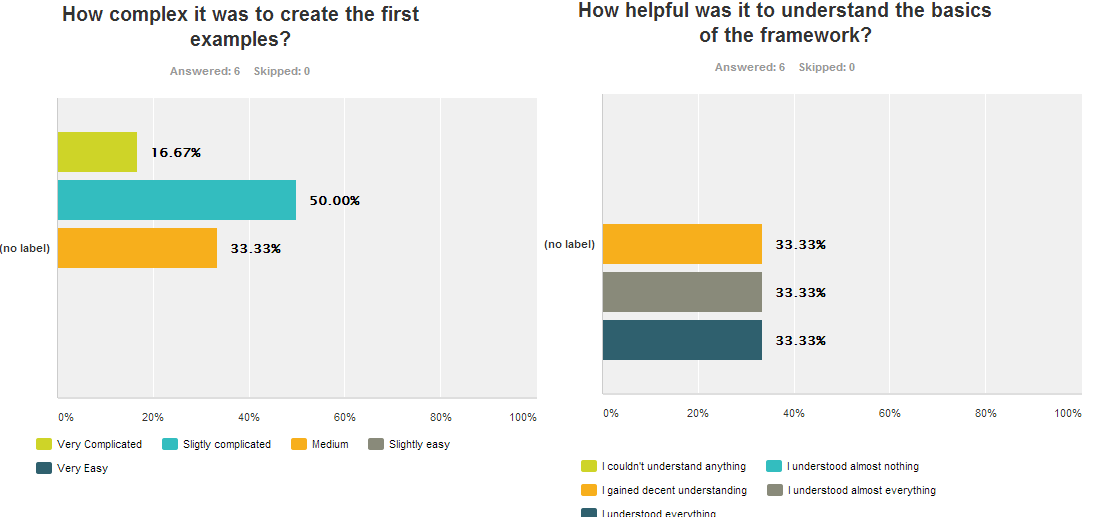
\includegraphics[scale=0.5]{Figures/q1.png}
\caption{Plotted answers to the question: "How complex it was to create the first examples?" and "How helpful was it to understand the basics of the framework?" }
\label{fig:firstex}
\end{figure}

For the GUI the results from participants were quite positive. The main problems with the GUI were the lack of feedback in the case of an error and lack of automation
at the URL fields. Each of those problems was fixed by adding pop-up dialogues in case of a missing field, example for the \textit{Terminals} field was added and the
URL fields don't need \textit{http}.
%==============================================================================
\chapter{Problems Encountered and Future Development}
It has been a great journey developing this project and one that will hopefully continue further. Since the
beginning there have been many difficulties with the project mostly related with the meta-programming field
it's focused on. Finding sources and doing research has been problematic because development in the field  of genetic programming 
isn't on the same scale as other more popular fields in programming (e.g Machine Learning, Artificial Intelligence).
However the result from the project has motived me to continue explore genetic programming even more and expand the
framework.

\section{Problems}
\textbf{Multiple Technologies -} among the main issues with the project is the amount of technologies used. This meant each of them
had to be understand so quality development in the area can be done. The framework was related to web services, genetic programming,
code generation, GUI which meant extensive research in each areas so the correct libraries or frameworks can be chosen. The learning
curve was steep for the project however each of the fields became easier to work and understand after the basics were clear.
\paragraph{}
\textbf{Proof of Concept -} before the project reached any results it had a \textit{proof of concept} label. Exploring new fields and
expanding your knowledge in specific fields can be fun but it's hard when not a lot of information is presented. Three times during the
project I had to reach out to \texit{stackoverflow.com} for help related to issues I couldn't find anywhere on the web resolved. The first
time it was related to the way Cherrypy processed it's requests and responses. The second one was focusing on the problem of converting
DEAP individuals into executable code or AST. Later on I had to tackle the problem on my own since such a functionality wasn't introduced to DEAP.
However the developers from DEAP were kind enough to provide support for further questions and the code generation has spawned the possibility
for an open source contribution to the DEAP framework with an extension that converts DEAP individuals to AST's. The third time was related
to code execution in python and the way arguments were passed to a sub processed.

\section{Future Development}
Since the beginning of the project the development has been very ambitious and all
the goals that were set were accomplished. Which gave the opportunity to think a lot about
improvements for the framework - anything from re-factoring, improving features to adding
additional functionality.

\subsection{Improvements}
\textbf{Expand beyond symbolic regression} - throughout the project symbolic regression was 
used as a proof of concept so the framework functionality can be showed. However non mathematical
web services are harder to implement using the framework and this can be improved so cloning can be
more automated. This can be done by adding a better method for overriding at the evaluating web service
and tweaking the basic primitives sets by adding primitives for control flows.
\paragraph{}
\textbf{AST for code generation} - currently all the code that is generated is in string form and through
unit tests it was proved that it's working well however using string manipulation rather then manipulating ASTs
is not as robust. A good re-factoring plan is to do all the code generation with ASTs and keep generation from
strings as little as possible. This would also help for creating the base for an open source contribution to
the DEAP framework that adds the functionality for individuals to be converted to ASTs and/or executable python code.
\paragraph{}
\textbf{Asynchronous requests} - among the initial requirements of the project was using a cloud of evaluating
web services to evaluate individuals over the web hence improving the speed especially for more complex
individuals. However that idea is a small project on it's own and it was going to bring a lot of complexity to the project.
Since the core of \textit{Darwin} is completed it's a solid place to start from however for dealing with threads
and asynchronous requests python is not the best language to handle the issues, implementing it in C would be much better

\subsection{New Functionality}
\textbf{Improvement of web services} - improving web service performance using the framework was an initial requirement
in the project but due to complexity and time issues it was opt-out from the project. The concept can still be implemented
and used for improving current web services that the developer has created so improved web service can be compared by performance
speed, memory usage and stability to the target one. After certain threshold of improvement is reached there can be automatic deployment
of the generated improved web service.
\paragraph{}
\textbf{Using unit tests as fitness} - a way of measuring fitness can be a set of unit tests the individual needs to pass. This way
individual can be tested if certain functionality exists and hence force the genetic program to evolve towards an individual with
the required functionality. From that point a dynamic addition of unit tests can be included so functionality can be introduced through
the evolution of a program. Comparing it to biological evolution its like adding a new threat for an organism in its environment hence
the organism needs to adapt.




%==============================================================================
\chapter{Conclusion}

\section{Summary}
The aim of the project was to develop a tool that uses genetic programming for cloning web services. After
three sprints of development, system and usability testing, the project was a success. The tool was successful
in satisfying the clients requirements and in cloning part of WolframAlpha's functionality. It managed to create a base
for further development in the area. Hopefully Darwin will be 
used by the genetic programming community and help genetic programming projects in the university.

\section{Contribution}
Introduction



%==============================================================================
\bibliographystyle{plain}
\bibliography{report}

\end{document}